\section{Method}
\label{vlprompt:sec:method}

In this section, we introduce our method, \textbf{VLPrompt}.
Given an image $\mathcal{I} \in \mathbb{R}^{H \times W \times 3}$ and language description $\mathcal{T}$ generated from LLMs, we extract vision and language features from them to predict panoptic scene graph $\mathcal{G} = \{\mathcal{O}, \mathcal{R}\}$, \ie, $\mathcal{G} = \text{VLPrompt} (\mathcal{I}, \mathcal{T})$.
In $\mathcal{G}$:
\begin{itemize}
    \item $\mathcal{O} = \{o_i\}_{i=1}^{N}$ signifies $N$ objects segmented from the image $\mathcal{I}$.
    Each object is defined by $o_i = \{c, m\}$, where $c$ belongs to one of the predefined $C$ object categories, and $m$ is a binary mask in $\{0, 1\}^{H \times W}$ for this object.
    \item $\mathcal{R} = \{r_{i,j} \mid i,j \in \{1, 2, \ldots, N\}, i \neq j\}$ denotes relations with $r_{i,j}$ being the relation between $o_i$ and $o_j$. Each $r$ belongs to one of the predefined $K$ relation categories (or no relation), $N$ is the number of objects in the image. 
\end{itemize}

\begin{figure}[t]
    \centering
    % \fbox{\rule{0pt}{2in} \rule{1.0\linewidth}{0pt}}
    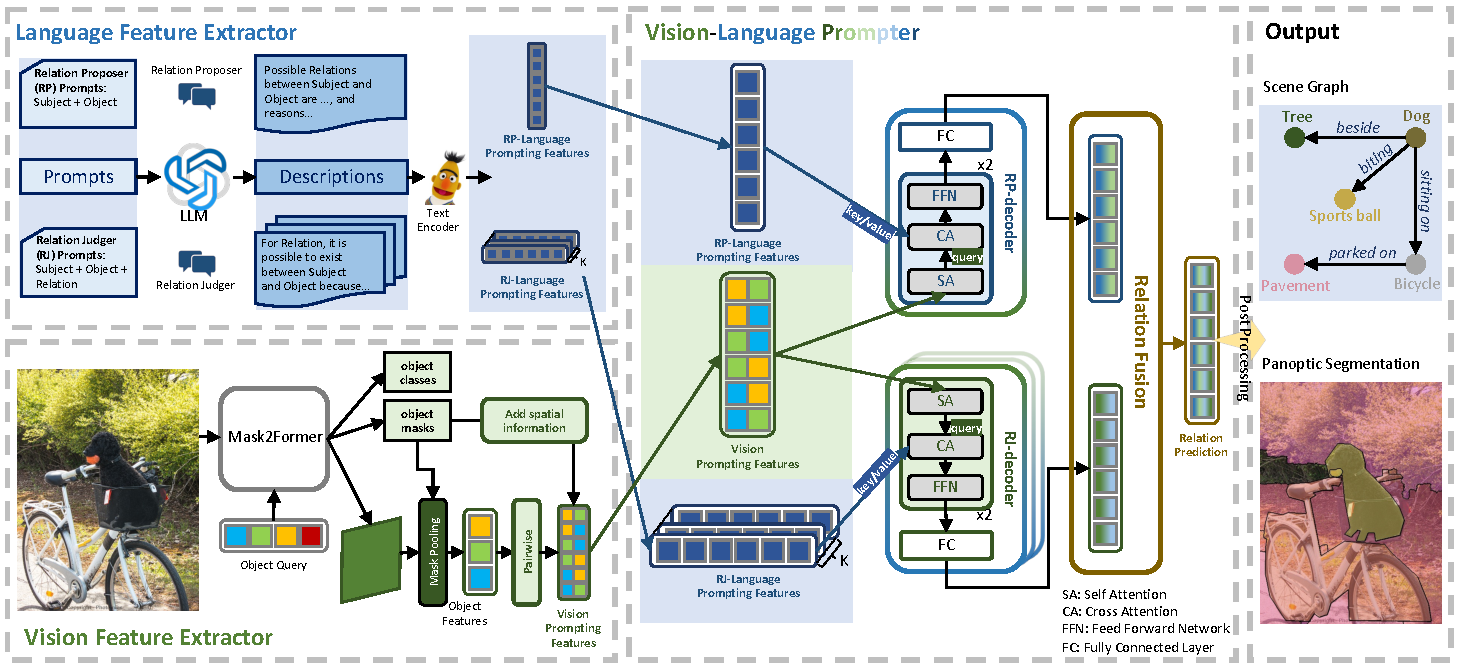
\includegraphics[width=1.0\linewidth]{Chapter4/Figures/overview_v3.pdf}
    \vspace{-4mm}
    \caption{The overall framework of VLPrompt, which comprises three components: the vision feature extractor, the language feature extractor and the vision-language prompter.
    We employ the language feature extractor to obtain LLM-based language information and integrate it into the final relation prediction through the vision-language prompter, enabling unbiased relation predictions.}
    \label{vlprompt:fig:overview}
\end{figure}

As shown in Fig.~\ref{vlprompt:fig:overview}, our method comprises three main components: \textit{vision feature extractor}, \textit{language feature extractor}, and \textit{vision-language prompter}.
The \textit{vision feature extractor} (Sec.~\ref{vlprompt:sec:vision_feature_extractor}) adapts from a segmentation network (\eg, Mask2Former~\citep{cheng2022masked}) to predict object masks and form subject-object pairs for feature extraction, which result into vision prompting features.
For the \textit{language feature extractor} (Sec.~\ref{vlprompt:sec:language_feature_extractor}), we generate different types of descriptions by leveraging the extensive common sense knowledge embedded in LLMs through carefully designed prompts, which is beneficial for relations of different frequencies.
These descriptions are then converted into language prompting features using a text encoder.
Next, the vision and language prompting features are fed into a \textit{vision-language prompter} (Sec.~\ref{vlprompt:sec:vision_language_prompter}), where vision prompting features interact with different types of language prompting features respectively, so as to take advantage of the complimentary language information to assist relation predictions. 
Finally, these relation predictions are combined by a relation fusion module to achieve the final relation prediction.


\subsection{Vision Feature Extractor}
\label{vlprompt:sec:vision_feature_extractor}

Given an image $\mathcal{I}$, we first leverage Mask2Former~\citep{cheng2022masked} to produce $N$ objects with masks.
They are formed into $N \times (N-1)$ subject-object pairs by pairing any two distinct ones. 
The purpose of the vision feature extractor is to extract vision prompting feature for each subject-object pair, which includes visual features from the segmentation network itself as well as spatial features between the subject-object pairs.
In this way, we can enhance the representations of the relations between subject-object pairs.  

\noindent \textbf{Subject-object visual features.}
We first obtain the features corresponding to each object.
Considering that the output feature map by the pixel decoder in Mask2Former retains rich information of the image, we use mask pooling to obtain object features corresponding to the $N$ objects from the feature map based on each object's mask $m$.
Then, we pair and concatenate any two distinct object features to form $N \times (N-1)$ subject-object visual features $F_{V}^{vi}$.

\noindent \textbf{Subject-object spatial features.}
To further enhance the representations of subject-object pairs, especially their spatial relations,  we are inspired by~\citet{peyre2017weakly} to encode the spatial features into the subject-object visual features.
Specifically, given $o_i$ and $o_j$ corresponding to subject and object, we first derive their encompassing bounding boxes $b_i=[x_i, y_i, w_i, h_i]$ and $b_j=[x_j, y_j, w_j, h_j]$, where $(x, y)$ is the center of the bounding box, and $(w, h)$ are the width and height.
Next we construct spatial features: 
\begin{equation}
    v(o_i, o_j) = [\frac{x_{j} - x_{i}}{\sqrt{w_{i}h_{i}}}, \frac{y_{j} - y_{i}}{\sqrt{w_{i}h_{i}}}, \sqrt{\frac{w_{j}h_{j}}{w_{i}h_{i}}}, \frac{b_i \cap b_j}{b_i \cup b_j}, \frac{w_i}{h_i}, \frac{w_j}{h_j}],
\end{equation}
where $v(o_i, o_j)$ encodes the spatial relation between $o_i$ and $o_j$, such as the ratio of their bounding box sizes, the overlap between two objects and the aspect ratio of each object.
Then, we use a FC layer to expand the spatial features to the same dimension as $F_{V}^{vi}$, resulting in $F_{V}^{sp}$.

Finally, we apply a FC layer to the sum of $F_{V}^{vi}$ and $F_{V}^{sp}$ and output vision prompting features $F_V \in \mathbb{R}^{N \times (N-1) \times D_{V}}$, where $D_{V}$ is the vision feature dimension.


\subsection{Language Feature Extractor}
\label{vlprompt:sec:language_feature_extractor}

The purpose of the language feature extractor is to leverage the extensive common sense knowledge embedded in LLMs for providing additional language information to the PSG task, which can mitigate the long-tail problem in relation prediction.
To achieve this, we need to design various prompts to elicit outputs from LLMs.
On one hand, LLMs can act as a relation proposer, suggesting possible relations between two objects, which often are frequently occurring relations in the real world.
On the other hand, LLMs can also serve as a relation judger, given a subject-object pair and their specific relation, LLMs make judgment and provide reasoning for this relation. This allows detailed descriptions even for rare relations.
Specifically, we design two types of prompts: relation proposer prompt (RP-Prompt) for proposing and explaining potential relations given a subject-object pair; relation judger prompt (RJ-Prompt) for judging and reasoning  upon a specific subject-relation-object triplet. 
Below, we detail how to obtain RP- and RJ-language prompting features based on the generated descriptions.

\noindent \textbf{RP-language prompting feature.}
For RP-language prompting feature, we stimulate LLMs to guess all possible relations between two given objects $o_i$ and $o_j$, along with explanation for these relations.
To achieve this, we utilize the chain-of-thought technique~\citep{wei2022chain}: we engage in a dialogue with an LLM (\eg, GPT-4~\citep{chatgpt}), initially informing it to act as a relation proposer and defining the task.
Then an example is provided to the LLM to clarify its role.
We explicitly mention the predefined $K$ relations in the prompt, guiding the LLM to propose from them.
Finally, a certain subject-object pair ($o_i$ and $o_j$) is given to the relation proposer prompt.
By giving this prompt to the LLM, we obtain the description for potential relations between $o_i$ and $o_j$.
For predefined relations that are not proposed by the LLM, we would append a template phrase by the end of the description, such as ``It is not likely for $o_i$ and $o_j$ to have relation $r$.'', to ensure that the language description clearly distinguishes common from uncommon relations and comprehensively covers all relation categories.
To encode the description into a feature interpretable by our model, we use a text encoder (\eg, OpenAI Embeddings~\citep{chatgpt}) to convert the description into the feature $F_{L(i, j)}^{RP} \in \mathbb{R}^{1 \times D_{L}}$, namely RP-language prompting feature.
This process consolidates all descriptions (each expressing multiple plausible relations for a given subject-object pair) into a single feature, allowing for a condensed reflection of the distinct attributes of common relations between subject and object.

\noindent \textbf{RJ-language prompting feature.}
For RJ-language prompting feature, we design the relation judger prompt: 
we not only provide two objects $o_i$, $o_j$ but also specify a relation $r_{k}$ between them. 
By using the common sense knowledge, the LLM judges whether the relation $r_{k}$ could plausibly exist between $o_i$ and $o_j$ and provides reason.
Similar to above, we use the chain-of-thought technique~\citep{wei2022chain} by telling the LLM that it serves as a relation judger; we first define the task, then give the example, and finally, the triplet ($o_i\text{-}r_{k}\text{-}o_j$) is provided.
Following the same process as for RP-language prompting feature, we feed the relation judger prompt to the LLM to obtain the language description and leverage the text encoder (same as above) to encode it into the RJ-language prompting feature $F_{L(i, j, k)}^{RJ} \in \mathbb{R}^{1 \times D_{L}}$. Different from the RP-language prompting feature, we encode each relation triplet into an individual feature, storing more detailed and subtle information for each relation, hence favouring rare relations.

By enumerating all $C$ objects and $K$ relations in the dataset, we derive all RP- and RJ-language prompting features.
To further enhance the practicality of our method and avoid repeatedly invoking LLM at runtime, we store them in a database.
Given an image with $N$ objects, we retrieve two sets of features, $F_{L}^{RP} \in \mathbb{R}^{N \times (N-1) \times D_{L}}$ and $F_{L}^{RJ} \in \mathbb{R}^{N \times (N-1) \times K \times D_{L}}$ from the database.
Note that for a specific relation $r_{k}$ between all subject object pairs in this image, the RJ-language prompting feature is denoted as $F_{L(k)}^{RJ} \in \mathbb{R}^{N \times (N-1) \times D_{L}}$.


\subsection{Vision-Language Prompter}
\label{vlprompt:sec:vision_language_prompter}

To enable the vision prompting feature to predict relations from both macro and detailed perspectives, we let $F_V$ interact with $F_L^{RP}$ and $F_L^{RJ}$ through two separate decoders, termed as RP-decoder and RJ-decoder, responsible for the interaction from $F_V$ to $F_L^{RP}$ and $F_L^{RJ}$, respectively. 
Each decoder contains two standard transformer decoder blocks~\citep{vaswani2017attention}, followed by a FC layer for relation prediction.
The predictions from the two decoders are complementary: the RP-language prompting feature focuses on the condensed and distinct attributes of frequently occurring relations for a given subject-object pair; in contrast, the RJ-language prompting feature focuses on the detailed and subtle attributes of every possible relation (common or rare) for the subject-object pair. A relation fusion module consisting of a gating network is thereby devised by the end to fuse the relation predictions from both decoders into the final one. Before feeding $F_V$, $F_L^{RP}$, and $F_L^{RJ}$ into different decoders, we use a FC layer to transform their dimensions to a uniform dimension $D$. Below, we specify the RP-decoder, RJ-decoder, and the relation fusion module, respectively.

\noindent \textbf{RP-decoder.}
The RP-decoder aims to utilize the $F_{L}^{RP}$ to assist $F_{V}$ in relation prediction, particularly for relations that are frequently encountered between $o_i$ and $o_j$ in the real world.
In the first transformer decoder block, $F_{V}$ is firstly fed into the self-attention layer, primarily aggregating the visual relational information in $F_{V}$.
Afterwards, the self-attended $F_{V}$ as query and the $F_{L}^{RP}$ as key/value are engaged in the subsequent cross-attention layer,
 aggregating the common sense knowledge of potential relations between $o_i$ and $o_j$ into $F_{V}$. 
The output is further processed through a feed-forward network.
In the second transformer decoder block, we repeat the aforementioned process.
Finally, a fully connected layer is used to transform feature dimension $D$ to the number of relations $K$, and a sigmoid function is applied afterwards to obtain $R^{RP} \in \mathbb{R}^{N \times (N-1) \times K}$. 

\noindent \textbf{RJ-decoder.}
The RJ-decoder aims to facilitate interaction between the RJ-language prompting feature $F_{L}^{RJ}$ with the vision prompting feature $F_{V}$.
Since $F_{L}^{RJ}$ a group of individual language prompting feature for every relation triplet ($o_i\text{-}r_{k}\text{-}o_j$), $F_V$ thus has the opportunity to interact with each relation's language representation independently, which can be particularly beneficial to rare relations.
We conduct parallel interactions between $F_V$ and the $K$ triplet features contained in $F_L^{RJ}$.
For each triplet, the interaction process between $F_V$ and $F_{L(k)}^{RJ}$ is the same to that of the RP-decoder, except that the final FC layer is now only responsible for predicting the probability of certain relation between $o_i$ and $o_j$. The FC layer is used to transform the feature dimension from $D$ to 1.
Finally, we concatenate the respective outputs to get the predictions for all $K$ relations, a sigmoid function is applied over them to obtain $R^{RJ} \in \mathbb{R}^{N \times (N-1) \times K}$.

\noindent \textbf{Relation Fusion.}
Upon obtaining $R^{RP}$ and $R^{RJ}$, we aim to take the strength of both via a relation fusion module.
We devise a gating network consisting of 3-layer MLP to generate two sets of weights, $W^{RP}$ and $W^{RJ}$, each matching the shape of $R^{RP}$ and $R^{RJ}$.
We use the sum of $F_V$ and $F_{L}^{RP}$ as the input of the gating network, and output $W^{RP}$.
For $W^{RJ}$, we use the sum of $F_V$ and the mean of $F_{L}^{RJ}$ along the relation dimension as input to the gating network.
$W^{RP}$ and $W^{RJ}$ are used to element-wisely multiply with $R^{RP}$ and $R^{RJ}$ respectively and the final relation prediction $R$ is a weighted combination:
\begin{equation}
    R = W^{RP} \odot R^{RP} + W^{RJ} \odot R^{RJ},
\end{equation}
where $\odot$ is element-wise multiplication, and $R \in \mathbb{R}^{N \times (N-1) \times K}$.

Finally, the prediction $R$, combined with the object categories and masks predicted by the vision feature extractor, forms the panoptic scene graph $\mathcal{G}$.


\subsection{Model Training}
\label{vlprompt:sec:model_training}
Our model training comprises two parts.
The first part is the segmentation loss $\mathcal{L}_{seg}$ used in the vision feature extractor for panoptic segmentation, we simply follow the loss used in~\citet{cheng2022masked}.
The second part is the relation loss. Since the same subject-object pair might have multiple relations, we use a binary cross-entropy loss~\citep{su2022zlpr}.
To effectively train the vision-language prompter, we apply the relation loss separately to $R^{RP}$, $R^{RJ}$, and $R$ and sum them up as the final relation loss, denoted by  $\mathcal{L}_{rel}$.
The final loss $\mathcal{L}$ is
\begin{equation}
    \mathcal{L} = \lambda \mathcal{L}_{seg} + \mathcal{L}_{rel},
\end{equation}
where $\lambda$ is the weighting coefficient.
In the language feature extractor, we directly utilize pre-trained LLMs, thus eliminating the need for additional model training.
